\documentclass[12pt, oneside]{article}
              		% See geometry.pdf to learn the layout options. There are lots.
\usepackage[margin=1in]{geometry}
\geometry{letterpaper}                   		% ... or a4paper or a5paper or ... 
%\geometry{landscape}                		% Activate for rotated page geometry
%\usepackage[parfill]{parskip}    		% Activate to begin paragraphs with an empty line rather than an indent
\usepackage{graphicx}				% Use pdf, png, jpg, or eps§ with pdflatex; use eps in DVI mode
								% TeX will automatically convert eps --> pdf in pdflatex		
\usepackage{amssymb}
\usepackage{ragged2e}

\graphicspath{ {pics/} }

%SetFonts

%SetFonts


\title{ECE 3150 Lab 1}
\author{Aalaap Narasipura}
\date{Febuary 26, 2016}							% Activate to display a given date or no date

\begin{document}
\maketitle
\begin{center}
Partner: Tim Braren
\end{center}
\section{Prelab}
\subsection{}
\begin{center}
\includegraphics[scale=.3]{exp_amp}\\
$V_{out}(t)=-Ae^{\frac{qV_{in}(t)}{\eta KT}}$\\$I=I_o(e^{\frac{qV_{in}(t)}{\eta KT}}-1)$\\
$-Ae^{\frac{qV_{in}(t)}{\eta KT}}=-V_{in}(t) \frac{R_2}{R_{in}}=I_{in}*R_2$\\
$-Ae^{\frac{qV_{in}(t)}{\eta KT}}=-I_oR_2e^{\frac{qV_{in}(t)}{\eta KT}}$\\
$-A=I_oR_2\rightarrow A=I-oR_2$
\end{center}
\subsection{}
\begin{center}
$V_{in}(t)=V_{in-DC}+V_{in-1}cos(n\omega t)$\\
$V_{out}(t)=-Ae^{\frac{qV_{in}(t)}{\eta KT}}=V_{out-DC}+\sum\limits_{\infty}^{n=1}V_{out-n}cos(n\omega t)$\\
$V_{out}=-I_oR_2e^{\frac{q(V_{in-DC}+V_{in-1}cos(n\omega t))}{\eta KT}}$\\
$V_{out}=-I_oR_2e^{\frac{q(V_{in-DC})}{\eta KT}}+e^{\frac{q(V_{in-1}cos(n\omega t))}{\eta KT}}$\\
$V_{out}=-I_oR_2e^{\frac{q(V_{in-DC})}{\eta KT}})(I_o\frac{qV_{in}}{\eta KT}+2\sum\limits_{\infty}^{n=1}I_n\frac{qV_{in-1}}{\eta KT}cos(n\omega t))$\\
$V_{out-DC}=-I_oR_2(e^{\frac{q(V_{in-DC})}{\eta KT}})(I_o\frac{qV_{in-1}}{\eta KT})$\\
$V_{out-n}=-I_oR_2(e^{\frac{q(V_{in-DC})}{\eta KT}})(2I_n\frac{qV_{in-1}}{\eta KT})$\\
$V_{out-1}=-I_oR_2(e^{\frac{q(V_{in-DC})}{\eta KT}})(2I_1\frac{qV_{in-1}}{\eta KT})$
\end{center}
\subsection{}
$(\frac{V_{out-n}}{V_{out-1}})^2=(\frac{-I_n(e^{\frac{q(V_{in-n})}{\eta KT}})}{-I_1(e^{\frac{q(V_{in-1})}{\eta KT}})})^2$
\\After plugging into Matlab the values obtained are:\\
$n=2\rightarrow -6.78dB$\\
$n=3\rightarrow -16.58dB$\\
$n=4\rightarrow -28.39dB$\\
$n=5\rightarrow -44.87dB$\\
\section{Post Lab Work}
\subsection{Diode Current-vs-Voltage (IV) Curve}
\begin{center}
\includegraphics[scale=.5]{VC}
\end{center}
The Diode Equation given by: $I=I_o(e^{\frac{qV_{in}(t)}{\eta KT}}-1)$ fitted very well to the measured data. The fitting values $\eta$ and $I_o$ were found by varying each one independently till the curve fit. I started with $\eta$ because it controlled the slope of the line. Once the slope matched the measured value I adjusted the value of $I_o$ till it match the measured slope The values that ended up working were $\eta = 1.94$ and $I_o = 4.2*10^-9$ Amps
\subsection{Large Signal Input and Output Waveforms}
\begin{center}
 Resistance Values\\
 \begin{tabular}{||c | c | c||} 
 \hline
 Resistor & Ideal $\Omega$ & Measured $\Omega$\\ 
 \hline
 R1 & 50 & 47.2\\
 \hline
 R2 & 100k & 97.7k\\
 
 \hline
\end{tabular}
\end{center}
The AC amplitude was found by looking at the peak to peak voltage on the oscilloscope and dividing that value by 2 to get the amplitude. The DC offset was found by looking at the oscilloscope.
\begin{center}
 DC offset $V_{in}$ and AC amplitude ($v_{1}$)\\
 \begin{tabular}{||c | c | c||} 
 \hline
   & Ideal $V_{in}$ (mV)& $v_{1}$ (mV)\\ 
 \hline
 CH1 & 290 & 68\\
 \hline
 CH2 & -222 & 240\\

 \hline
\end{tabular}
\end{center}
\begin{center}
\includegraphics[scale=.5]{wave}
\end{center}
The measured and calculated outputs for the waveform vs. time were very similar. Our calculated output ended up being a bit higher than what we measured, which can be due to outside noise and the fact that the devices we are using are not ideal. We did get the waveforms we wanted with a fairly low margin of error.

\subsection{Large Signal Input and Output FFT Spectra}
\begin{center}
\includegraphics[scale=.5]{db}
\end{center}
The measured and calculated values for the harmonic peaks were close. They both followed the downward dB as the index n got higher. Our measured values ended up being lower by approximately 10dB than the calculated one. We obtained the calculated values by using the Bessel function. Following what we did in the prelab in order to get the calculated values. We did get a new calculated value of $\eta$ being 1.94. In the measured data the $5^{th}$ harmonic ended up being more off than the other harmonics. This is due to the fact that the magnitude of $5^{th}$ harmonic was very close to the surrounding noise. Thus, the noise messes with the signal more here which contributed to the higher margin of error.


\subsection{Small Signal Measurements: Diode Differential Resistance}
\begin{center}
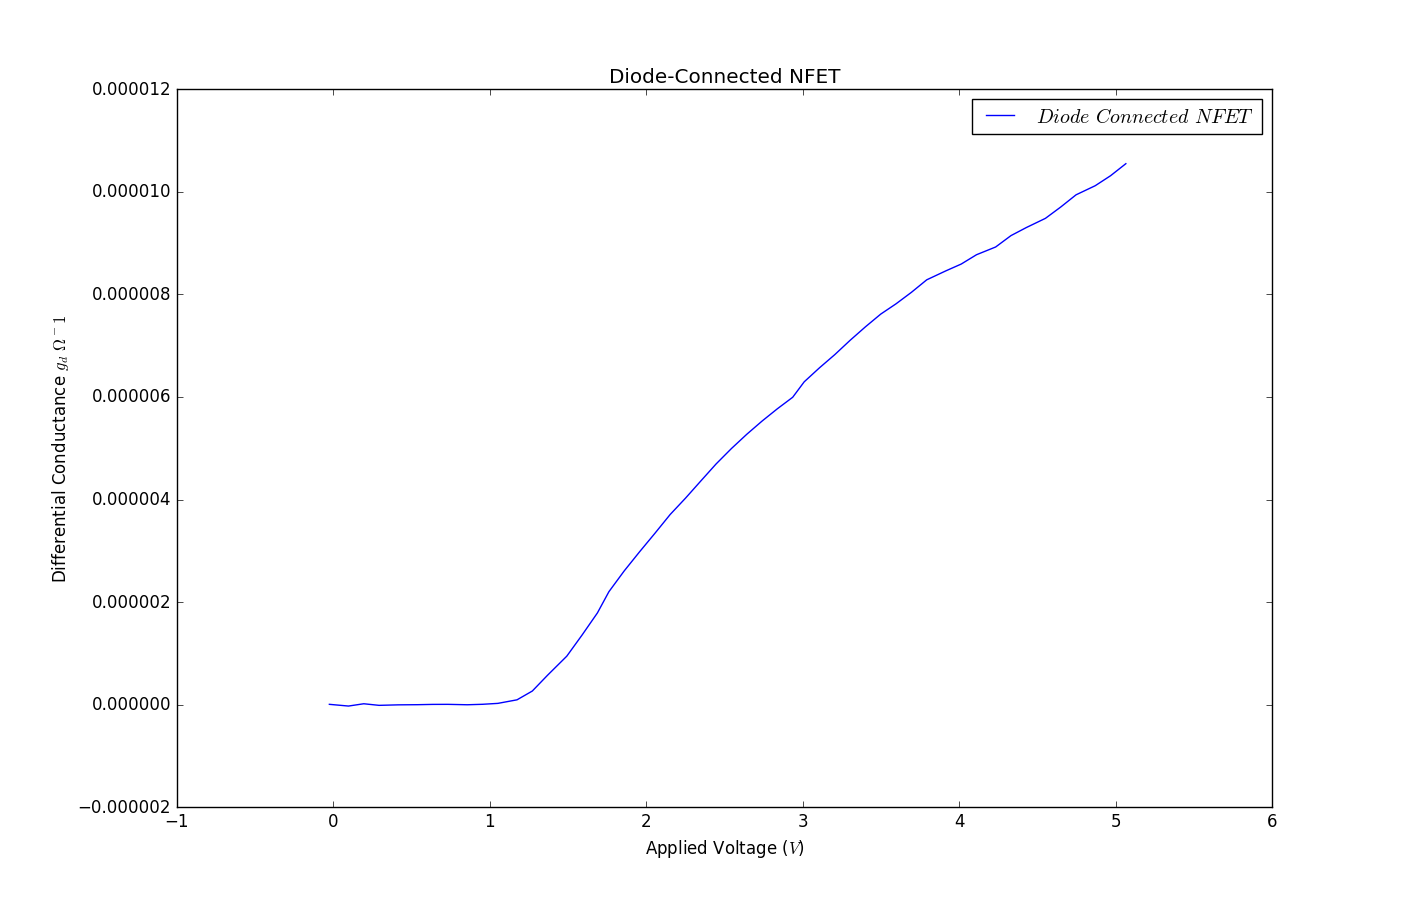
\includegraphics[scale=.7]{figure_1}
\end{center}
At the input DC bias voltage of 400mv the differential resistance was 3.203k$\Omega$.

\subsection{Small Signal Measurements: Circuit Gain}
\textbf{a)}\\
The small circuit model of the op-amp exponential amplifier behaves very similar to an ideal op-amp. Thus we can use the derive the voltage gain using the formula for an ideal op amp. $V_{out}=-V_{in}\frac{R_f}{R_{in}}$. This modified for our op-amp changes the equation to be: $V_{out}=-V_{in}\frac{R_2}{r_{d}} \rightarrow \frac{V_{out-1}}{V_{in-1}}=\frac{-R_2}{r_d}\rightarrow A_v=\frac{-R_2}{r_d}$ Where $r_d$ is the diode differential resistance.\\
\begin{center}
\includegraphics[scale=.7]{gain}
\end{center}

\begin{center}
 \begin{tabular}{||c | c | c||} 
 \hline
   & Voltage Bias & Gain\\ 
 \hline
 Theoretical & 400mv & 29.2\\
 \hline
  Theoretical & 500mv & 176.98\\

 \hline
 Measured & 400mv & 4\\
 \hline
  Measured & 500mv & 19\\
 
 \hline
\end{tabular}
\end{center}

\begin{center}
 \begin{tabular}{||c | c | c||} 
 \hline
   \textbf{400mv} & DC Offset [mV] & Pk-to-Pk[mv]\\ 
 \hline
 CH1 & 286 & 2\\
 \hline
  CH2 & -131 & 8\\
  \hline
  \textbf{500mv}& &  \\

 \hline
 CH1 & 312 & 2\\
 \hline
  CH2 & -236 & 38\\
 
 \hline
\end{tabular}
\end{center}
\textit{The AC signal amplitude setting on the function generator was 19mV at onset of linear operation}\\
\textbf{b)}\\
The ideal gain using the measured values would be $4.84$ for 400mv and $35.74$ for 500mv
The measure gain was quite a bit off from the theoretical values. The main reason for this was that because we running at such a small voltage, the outside noise was very noticeable and messed with the measurements. In lab when we first connected the input voltage we got a high gain initially but it then flat lined to the value we ended up using to calculate the gain. However, our gain did increase from the 400mv measurement to the 500mv measurement. This is consistent with the fact that the differential resistance calculated in \textbf{2.4} decreases as with an increase in the bias voltage.

\end{document}  